\chapter{ПРАКТИЧЕСКАЯ РАБОТА № 2 <<СТРУКТУРНЫЙ АНАЛИЗ И ПРОЕКТИРОВАНИЕ ПРОГРАММНЫХ СИСТЕМ>>)}

\section{Цель работы}

Провести структурный анализ и построить DFD-диаграммы для заданной предметной области. Одна диаграмма должна представлять обобщенную работу системы, одна --- детализацию одного из процессов (обе диаграммы должны включать 5-7 процессов). Построить STD-диаграмму системы.

\section{Краткие теоретические сведения}

Понятие жизненного цикла (ЖЦ) программного обеспечения (ПО) регламентирует основные процессы его разработки и эксплуатации. ЖЦ формулируется как модель создания и использования ПО, отражающая его различные состояния, начиная с момента возникновения необходимости в данном программном изделии и заканчивая моментом его полного выхода из употребления у всех пользователей.

В  ЖЦ ПО выделяются следующие основные этапы:

\begin{enumerate}
	\item{Анализ требований и постановка задачи.}
	\item{Анализ и исследование задачи, модели, проектирование.}
	\item{Кодирование (программная реализация).}
	\item{Тестирование и отладка.}
	\item{эксплуатация и сопровождение.}
\end{enumerate}

ЖЦ образуется в соответствии с принципом нисходящего проектирования и, как правило, носит итерационный характер: реализованные этапы, начиная с самых ранних, циклически повторяются в соответствии с изменениями требований и внешних условий, введением ограничений и т.п. На каждом этапе ЖЦ порождается определенный набор документов и технических решений, при этом для каждого этапа исходными являются документы и решения, полученные на предыдущем этапе. Каждый этап завершается верификацией порожденных документов и решений с целью проверки их соответствия исходным.

Модель ЖЦ формулирует порядок исполнения этапов в ходе разработки, а также правила перехода от одного этапа к другому. На литературе по программной инженерии выделяют следующие модели как основные вехи в истории развития принципов анализа:

\subsection{Каскадная модель}

Каскадная модель была предложена Уинтсоном Ройсом в 1970 году. Эту модель принято называть классической и она предполагает, что  переход на следующий этап после полного окончания работ по предыдущему этапу.

К преимуществам каскадной модели относят:

\begin{enumerate}
	\item{Четкую регламентацию выполнения этапов проекта.}
	\item{Возможность оценки качества продукта на каждом из этапов.}
\end{enumerate} 

В то же время у этой модели имеются существенные недостатки:

\begin{enumerate}
	\item{Модель не предусматривает  обратных связей между этапами.}
	\item{Она не соответствует реальным условиям разработки программного продукта.}
\end{enumerate} 

\subsection{Поэтапная модель с промежуточным контролем}

Поэтапная модель с промежуточным контролем --- итерационная модель разработки ПО с циклами обратной связи между этапами. Преимущество такой модели заключается в том, что межэтапные корректировки обеспечивают меньшую трудоемкость по сравнению с каскадной моделью; с другой стороны, время жизни каждого из этапов растягивается на весь период разработки.

В этой модели предусмотрен промежуточный контроль за счет обратных связей. По итогам каждого из этапов возможен откат на предыдущий (-ие) шаги в случае, если выход этапа плохо верифицируем или в процессе разработки изменились исходные требования к системе.  При работе с реальным проектом в классической каскадной модели обычно возникают проблемы при обнаружении недоработок и ошибок, допущенных на ранних этапах. Стройность процесса разработки нарушают также изменениями окружения, в котором разрабатывается ПО, такие как изменения требований заказчика, изменения политик разрабатывающей или эксплуатирующей организации, изменения отраслевых стандартов, появление конкурирующих продуктов и пр. Подобные нелинейности в процессе разработки учитываются в модели с промежуточным контролем. Недостатком поэтапной модели в сравнении с классической можно назвать существенное (до 10 раз) увеличение затрат на реализацию проекта.

\subsection{Спиральная модель}

Спиральная модель --- делает упор на начальные этапы ЖЦ: анализ требований, проектирование спецификаций, предварительное и детальное проектирование. На этих этапах проверяется и обосновывается реализуемость технических решений путем создания прототипов.

Модель строится на четырех основных операциях, соответствующих квадрантам спирали:
\begin{enumerate}
	\item{Планирование --- определяет цели разработки, формулирует варианты решения и накладывает ограничения на работу системы;}
	\item{Анализ рисков --- заключается в оценке рисков для различных вариантов решения;}
	\item{Конструирование --- непосредственная разработка продукта на новом уровне;}
	\item{Оценивание --- предполагает оценку результатов, достигнутых на этапе конструирования.}
\end{enumerate}

Каждый виток спирали соответствует поэтапной модели создания фрагмента или версии программного изделия, на нем уточняются цели и характеристики проекта, определяется его качество, планируются работы следующего витка спирали. Таким образом, углубляются и последовательно конкретизируются детали проекта и в результате выбирается обоснованный вариант, который доводится до реализации. При этом на этапе конструирование на каждом витке спирали может включать полный каскад классического жизненного цикла.

Специалистами отмечаются следующие преимущества спиральной модели:
\begin{enumerate}
	\item{Накопление и повторное использование программных средств, моделей и прототипов;}
	\item{Ориентация на эволюционное развитие и модификацию ПО в процессе его проектирования;}
	\item{Позволяет оценивать риски и издержки в процессе проектирования на каждом витке эволюции разработки.}
\end{enumerate}
Недостатками спиральной модели можно считать сложность оценки времени процесса разработки и необходимость более тесного вовлечения заказчика в процесс разработки.


Главная особенность индустрии ПО состоит в концентрации сложности на начальных этапах ЖЦ (анализ, проектирование) при относительно невысокой сложности и трудоемкости последующих этапов. Более того, нерешенные вопросы и ошибки, допущенные на этапах анализа и проектирования, порождают на последующих этапах трудные, часто неразрешимые проблемы и, в конечном счете, приводят к неуспеху всего проекта.
\section{Заданная предметная область}

Антивирус-ревизор. Система фиксирует состояние заданных пользователем папок и в случае изменения их состояния (количество файлов, размер, дата создания или модификации, атрибуты) отмечает измененные элементы файловой системы как подозрительные. Проверка состояния папок осуществляется либо по расписанию, либо команде пользователя.

\section{Выполнение практической работы}

\subsection{Диаграмма обобщенной работы системы}

\begin{figure}[h!]
	\centering
	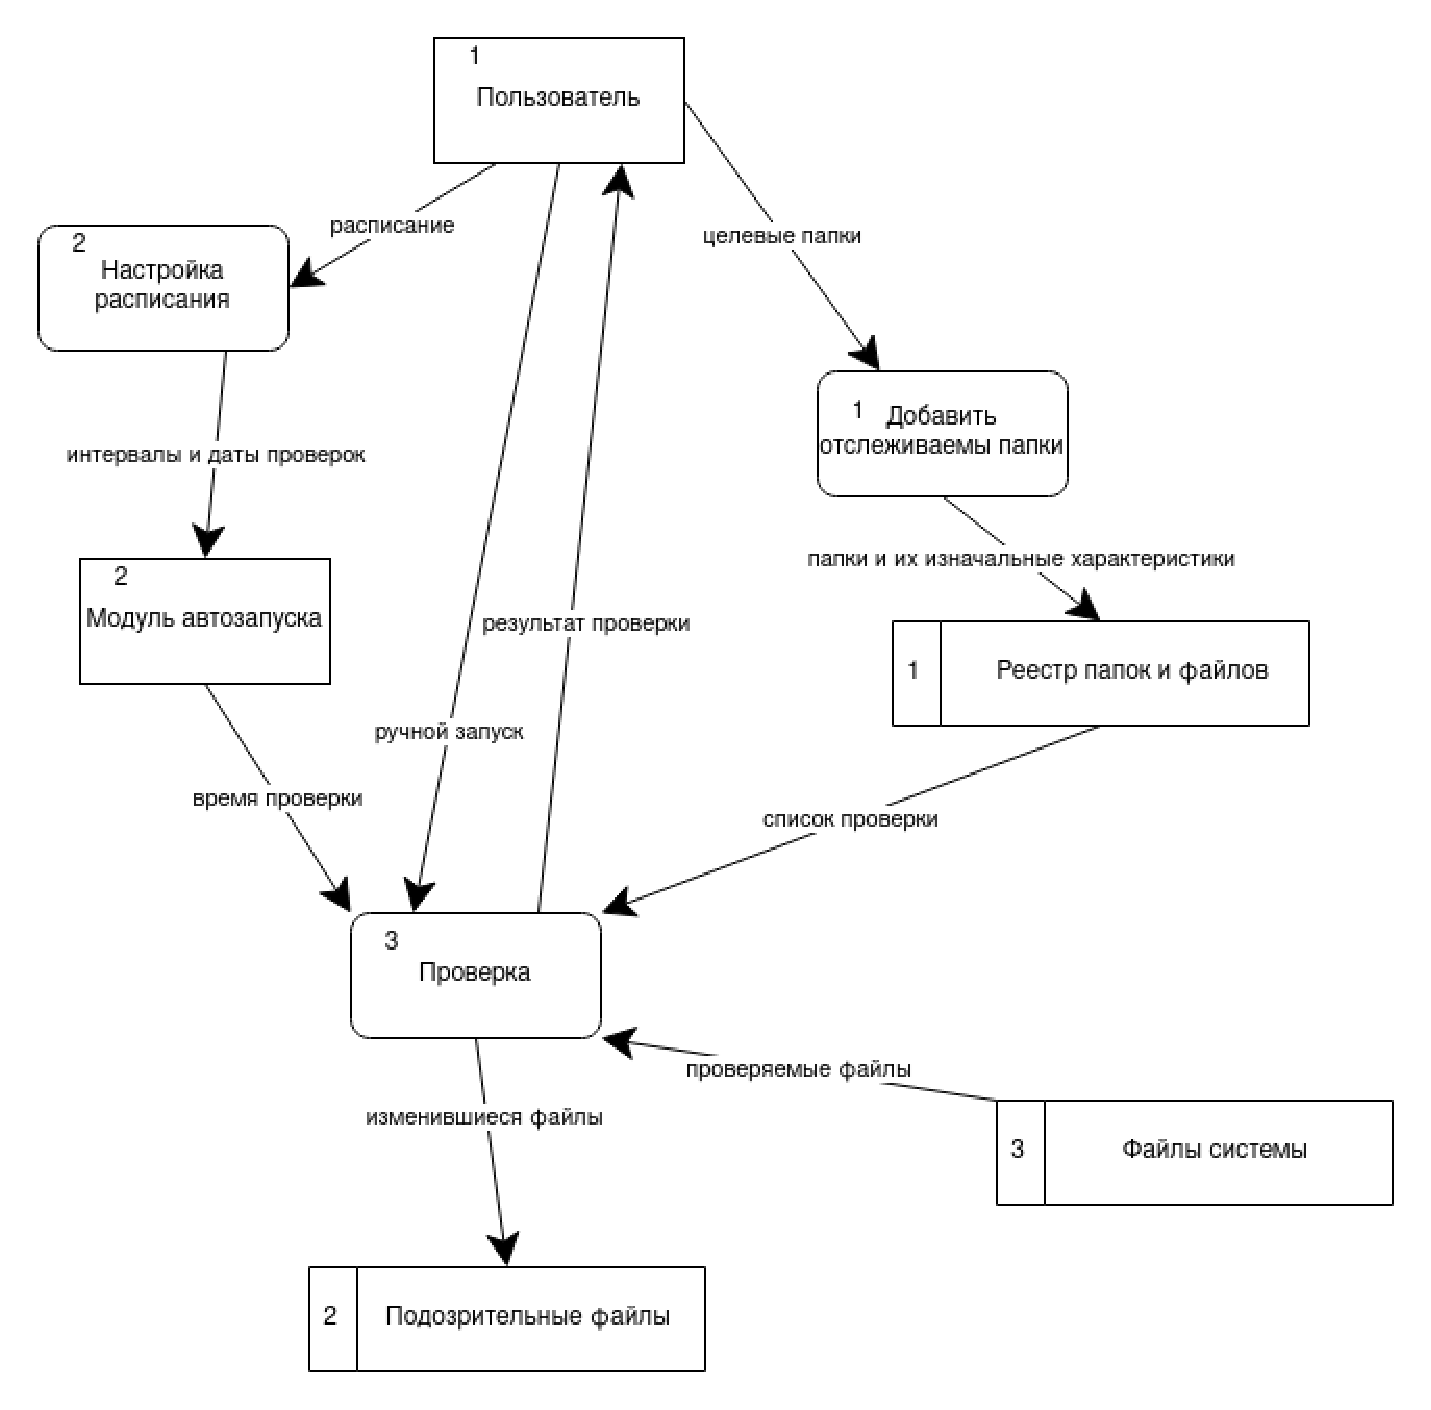
\includegraphics[width=0.5\textwidth]{images/2/total.eps}
	\caption{Диаграмма обобщенной работы системы}
\end{figure}

\subsection{Детализация процесса системы}



\subsection{STD-диаграмма системы}

\begin{figure}[h!]
	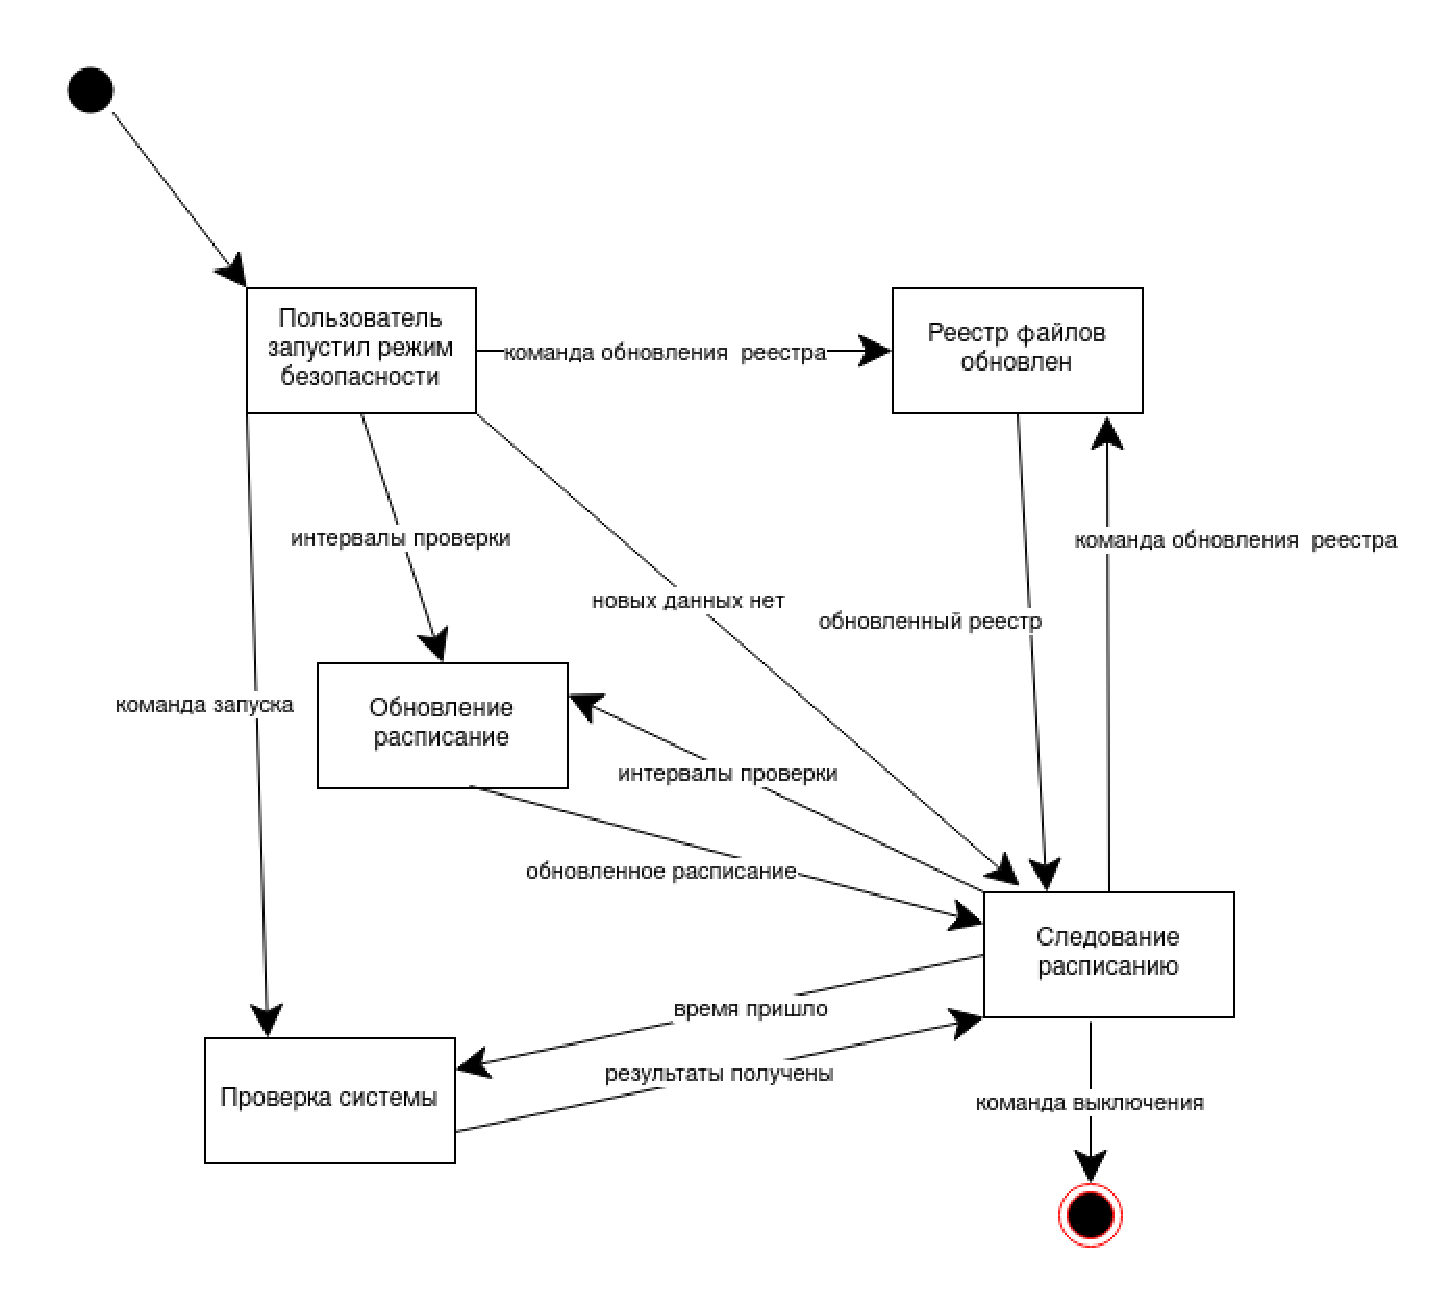
\includegraphics[width=0.8\textwidth]{images/2/std.eps}
	\caption{STD-диаграмма системы}
\end{figure}
\section{Вывод}

Был проведен структурный анализ и пострены DFD-диаграммы для заданной предметной области. 
